
%%% Local Variables:
%%% mode: latex
%%% TeX-master: t
%%% End:

\documentclass[xcolor=svgnames,11pt]{beamer}
\usepackage[utf8]{inputenc}
\usepackage[english]{babel}
\usepackage{hyperref}
\usepackage{mathrsfs}
\usepackage{geometry}
\usepackage{listings}
\usepackage{graphicx}
\usepackage{xspace}
\usepackage{verbatim}
\usepackage{textcomp}
\usepackage{amsmath}
\usepackage{amsfonts}
\usepackage{syntax}
\usepackage{amssymb}
\usepackage{mathtools}
\usepackage{subcaption}
\usepackage{textgreek}
\usetheme{Frankfurt}
\usecolortheme{crane}

\beamertemplatenavigationsymbolsempty
\usepackage{tikz}
\usetikzlibrary{backgrounds,positioning,shapes,shadings,shadows,arrows,decorations.markings,calc,fit,fadings}
\input{../tikz}

\newcommand{\coq}{\textsc{Coq}\xspace}
\newcommand{\agda}{\textsc{Agda}\xspace}
\newcommand{\ma}{\textsc{microAgda}\xspace}
\newcommand{\na}{\textsc{nanoAgda}\xspace}

\lstset{
  tabsize=4,
  aboveskip={0.4\baselineskip},
  belowcaptionskip=0.4\baselineskip,
  columns=fixed,
  showstringspaces=false,
  extendedchars=true,
  breaklines=true,
  frame=none,
  xleftmargin=\parindent,
  basicstyle=\footnotesize\ttfamily,
  keywordstyle=\bfseries\color{green!30!black},
  keywordstyle=[2]\bfseries\color{red!50!white},
  commentstyle=\itshape\color{purple!40!black},
  identifierstyle=\color{blue!30!black},
  stringstyle=\color{orange},
}

\lstdefinelanguage{Agda}{
  morekeywords={data,where,case,let,in},
  literate={->}{{$\to{}$}}1 {xx}{{$\times$}}1 {==}{{$\equiv$}}1 {*}{{$\times$}}1,
}

\lstdefinelanguage{nanoAgda}{
  morekeywords={case,of,split,rec},
  literate={->}{{$\to$}}1 {\\}{{$\lambda$}}1 {'}{`}1
    {*}{{$\times$}}1 {*0}{{$\star_0$}}2 {*1}{{$\star_1$}}2 {*2}{{$\star_2$}}2,
}
\lstset{
  aboveskip=0pt,
  belowcaptionskip=0pt,
  basicstyle=\small\ttfamily,
  escapeinside={!}{!},
}


\title{A sequent-calculus presentation of type-theory}
\author[Gabriel Radanne]{Gabriel Radanne --- Under the supervision of Jean-Philippe Bernardy}
\institute[ENS Rennes]{ENS Rennes --- Chalmers University of Technology}

\begin{document}

\begin{frame}[plain]
\titlepage
\end{frame}

\begin{frame}{Plan}
\tableofcontents%[section]
\end{frame}

\section{An Introduction to dependent types}

\begin{frame}{Dependent types}

\end{frame}

\begin{frame}{A crash course into dependent types}
The example from the report, maybe a bit shortened
\end{frame}

\section{Limitations of current typecheckers}

\subsection{Efficiency issues}
\begin{frame}{Efficiency issues}
  \agda's type checker uses a natural deduction style:
  \begin{itemize}
  \item Inference duplicates parts of terms.
  \item These parts are not shared in the \agda core representation anymore.
  \item Typechecking must be done multiple time, causing performance penalties.
  \end{itemize}
  \pause
  \begin{figure}
    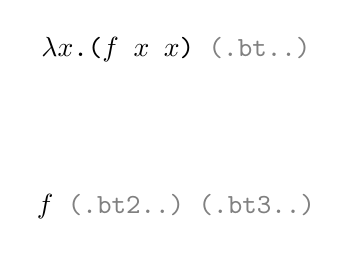
\begin{tikzpicture}
      \node[anchor=center] (lambda) at (0,0) {
        \texttt{$\lambda{}x$.($f$ $x$ $x$) {\color{Gray}(.\tikzcoord{bt}..)}}
      };
      \node<3>[anchor=center, text centered] (lambda2) at (0,-2) {
        \texttt{$f$\ {\color{Gray}(.\tikzcoord{bt2}..)\ (.\tikzcoord{bt3}..)}}
      };
    \end{tikzpicture}
    \centering
  \end{figure}
  \begin{tikzpicture}[remember picture, overlay]
    \node[xshift=0.1cm,yshift=-0.2cm, coordinate] (bt') at (bt) {} ;
    \draw<3>[remember picture, -latex] (bt') to[out=-90,in=90] ($(bt2)+(0.1,0.3)$) ;
    \draw<3>[remember picture, -latex] (bt') to[out=-90,in=90] ($(bt3)+(0.1,0.3)$) ;
  \end{tikzpicture}
\end{frame}

\subsection{The ``case decomposition'' issue}
\begin{frame}{The ``case decomposition'' issue}
  Natural deduction style makes propagating typing constraints to subterms difficult.

  For example, \agda's typechecker has no knowledge of which branch was taken while it typechecks the body of a case.
  \begin{center}
    \begin{minipage}{0.9\textwidth}
      \lstinputlisting[basicstyle=\ttfamily,language=Agda]{../poster/case.agda}
    \end{minipage}
  \end{center}
\end{frame}

\subsection{The monolithic approach}
\begin{frame}{The monolithic approach}
  \agda currently does not have a core language that can be reasoned about and formally verified.

  \coq, on the other hand, is built as successive extensions of a core language (CIC).
  \begin{figure}[htbp]
    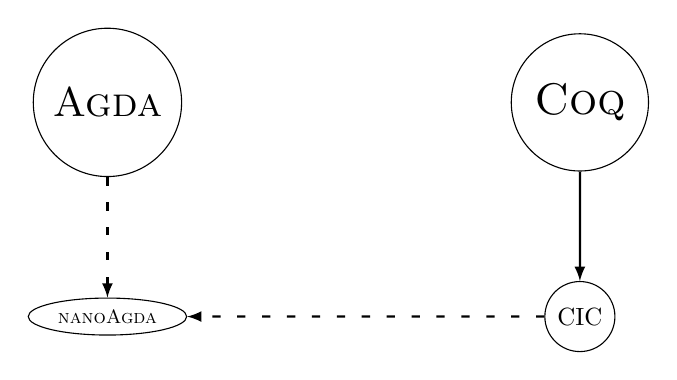
\begin{tikzpicture}[yscale=0.4, xscale=0.4]
      \node[draw, circle, scale=1.6] (Coq) at (8,3) {\coq} ;
      \node[draw, circle, scale=0.9] (CCC) at (8,-3.8) {CIC} ;
      \node[draw, circle, scale=1.5] (agda) at (-7,3) {\agda} ;
      % \node[draw, ellipse, scale=0.9] (ma) at (-7,3) {\ma} ;
      \node<3>[draw, ellipse, scale=0.7] (na) at (-7,-3.8) {\na} ;
      \draw[-latex,thick] (Coq) -- (CCC) ;
      % \draw[-latex,thick] (ma) -- (na) ;
      \draw<3>[-latex,thick, loosely dashed] (agda) to (na) ;
      \draw<3>[-latex,thick, loosely dashed] (CCC) to (na) ;
    \end{tikzpicture}
    \centering
  \end{figure}
\end{frame}

\section{\na and \ma}

\subsection{Goals}
\begin{frame}{Goals}
  Our goals are to have a language that is:
  \begin{itemize}
  \item<1-> A type-theory: Correctness should be expressible via types.
  \item<2-> Low-level: One should be able to translate high-level languages into this language while retaining properties such as run-time behaviour, complexity, etc.
  \item<3-> Minimal: The language should be well defined and it should be possible to formally verify the type-checking algorithm.
  \end{itemize}
\end{frame}

\subsection{\na}
\begin{frame}{\na}
Some introductory example of \na
\end{frame}

\begin{frame}{Sequent calculus}
Explanation of why Sequent calculus will solve all the problems in the (type theory) word.
\end{frame}

\begin{frame}[shrink]{Presentation of the language}
\begin{figure}[!h]
  \begin{subfigure}[b]{0.3\linewidth{}}
    \begin{align*}
      \ensuremath{\text{t}} ::=\:&\ensuremath{\overline{\text{x}}}\\ |\:&\ensuremath{\text{\texttt{let}}\:\text{x}=\text{d}\:\text{\texttt{in}}\:\text{t}}\\ |\:&\ensuremath{\text{\texttt{case}}\:\text{x}\:\text{\texttt{of}}\:\{\text{\ensuremath{(\text{`l}\to{}\text{t})}\ensuremath{\text{*}}}\}}\\ |\:&\ensuremath{\text{\texttt{let}}\:\overline{\text{x}}=\text{c}\:\text{\texttt{in}}\:\text{t}}
    \end{align*}
    \caption{Terms}
  \end{subfigure}
  \begin{subfigure}[b]{0.25\linewidth{}}
    \begin{align*}
      \ensuremath{\text{d}} ::=\:&\ensuremath{\text{x}} \: \ensuremath{\overline{\text{y}}}\\ |\:&\ensuremath{\text{x}\mathsf{.1}} \: | \: \ensuremath{\text{x}\mathsf{.2}} \\ |\:&\textcolor{red}{\ensuremath{\overline{\text{x}}:\overline{\text{y}}}}
    \end{align*}
    \caption{Destructions}
  \end{subfigure}
  \begin{subfigure}[b]{0.3\linewidth{}}
    \begin{align*}
      \ensuremath{\text{c}} ::=\:&\ensuremath{\text{x}}\\|\:&\ensuremath{\lambda{{}}} \ensuremath{\text{x}} . \ensuremath{\text{t}}\:|\:\ensuremath{(\text{x}:\overline{\text{y}})\to{}\text{t}}\\|\:&(\ensuremath{\overline{\text{x}}},\ensuremath{\overline{\text{y}}})\:|\:\ensuremath{(\text{x}:\overline{\text{y}})\times{}\text{t}}\\|\:&\ensuremath{\text{`l}}\:|\:\ensuremath{\{\text{`l}\}}\\|\:&\ensuremath{\star{}} \ensuremath{_{\text{i}}}
    \end{align*}\caption{Constructions}
  \end{subfigure}
\end{figure}
\end{frame}


\section{Future work}



\end{document}
